\documentclass[border=0.5mm]{standalone}
\usepackage{tikz}
\usetikzlibrary{arrows.meta, positioning}

\begin{document}

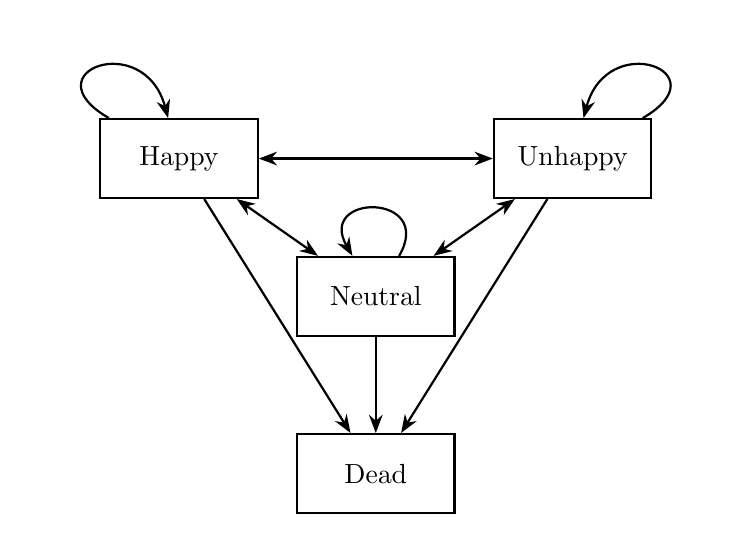
\begin{tikzpicture}[
    % Define node style
    node style/.style={
        draw, % Draw border
        rectangle, % Rectangle shape
        minimum width=2cm, % Minimum width
        minimum height=1cm, % Minimum height
        align=center % Center alignment
      },
    % Define arrow style
    ->, % Default arrow direction
    >=Stealth, % Arrow type
    thick % Line thickness
  ]

  % Define nodes
  \node[node style] (Happy) at (-2.5, 1.5) {Happy}; % Node h on the left, height at 1
  \node[node style] (Unhappy) at (2.5, 1.5) {Unhappy};  % Node u on the right, height at 1, same level as h
  \node[node style] (Neutral) at (0, -0.25) {Neutral}; % Node n in the middle, between h/u and d
  \node[node style] (Dead) at (0, -2.5) {Dead}; % Node d at the bottom, below the middle of h and u

  % Draw arrows and labels
  % p_hh: self-loop arrow, keep curved
  \draw[->] (Happy) to[out=150, in=105, looseness=4] (Happy);

  % p_hu & p_uh: bidirectional arrow between h and u
  \draw[<->] (Happy) -- (Unhappy);

  % p_uu: self-loop arrow, keep curved
  \draw[->] (Unhappy) to[out=30, in=75, looseness=4] (Unhappy);

  % p_hn & p_nh: bidirectional arrow between h and n
  \draw[<->] (Happy) -- (Neutral);

  % p_un & p_nu: bidirectional arrow between u and n
  \draw[<->] (Unhappy) -- (Neutral);

  % p_nn: self-loop arrow for neutral above the state
  \draw[->] (Neutral) to[out=60, in=120, looseness=4] (Neutral);

  % p_hd: from h to d, straight
  \draw[->] (Happy) -- (Dead);

  % p_ud: from u to d, straight
  \draw[->] (Unhappy) -- (Dead);

  % p_nd: from n to d, straight
  \draw[->] (Neutral) -- (Dead);

\end{tikzpicture}

\end{document}
